\begin{figure}[H]
\centering
\begin{subfigure}[H]{0.4\textwidth}
	\centering

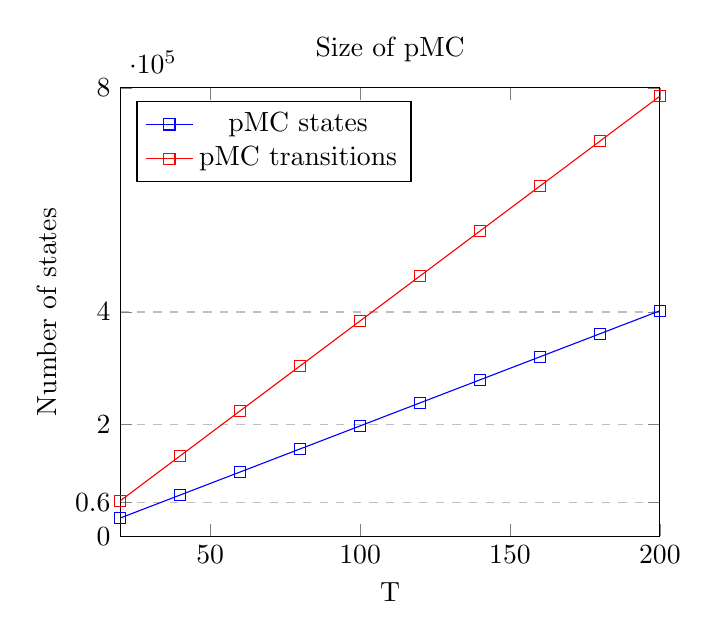
\begin{tikzpicture}
\begin{axis}[
    title={Size of pMC},
    xlabel={T},
    ylabel={Number of states},
    xmin=20, xmax=200,
    ymin=0, ymax=800000,
    xtick={0,50,100,150,200},
    ytick={0,200000,400000,60000,800000},
    legend pos=north west,
    ymajorgrids=true,
    grid style=dashed,
]

\addplot[
    color=blue,
    mark=square,
    ]
    coordinates {
    (20,32432)(40,73532)(60,114632)(80,155732)(100,196832)(120,237932)(140,279032)(160,320132)(180,361232)(200,402332)
    };
    
\addplot[
    color=red,
    mark=square,
    ]
    coordinates {
    (20,63222)(40,143442)(60,223662)(80,303882)(100,384102)(120,464322)(140,544542)(160,624762)(180,704982)(200,785202)
    };
    \legend{pMC states, pMC transitions}

\end{axis}
\end{tikzpicture}
\end{subfigure}
\hfill
\begin{subfigure}[H]{0.4\textwidth}
	\centering
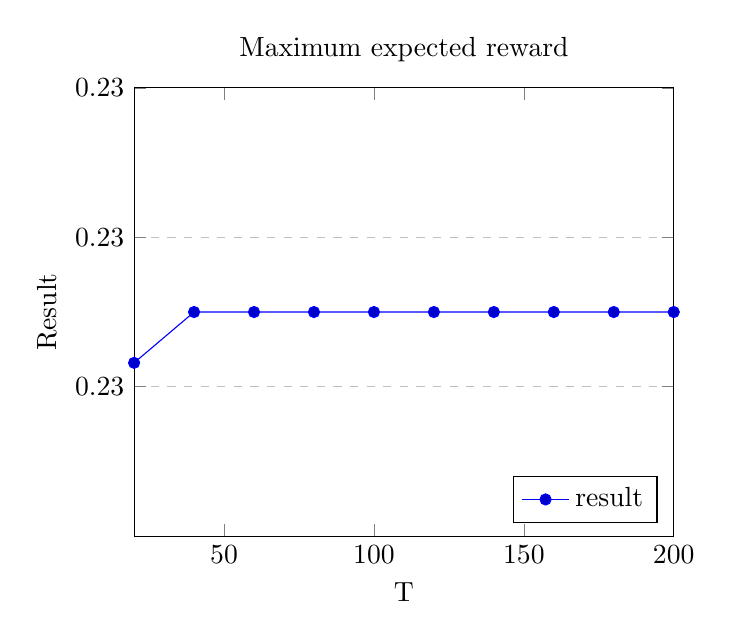
\begin{tikzpicture}

\begin{axis}[
    title={Maximum expected reward},
    xlabel={T},
    ylabel={Result},
    xmin=20, xmax=200,
    ymin=0.2255,ymax=0.227,
    xtick={0,50,100,150,200},
    ytick={0.226,0.2265,0.227},
    legend pos=south east,
    ymajorgrids=true,
    grid style=dashed]    
\addplot
    coordinates {
    (20,0.22608)(40,0.22625)(60,0.22625)(80,0.22625)(100,0.22625)(120,0.22625)(140,0.22625)(160,0.22625)(180,0.22625)(200,0.22625)
    };
    \legend{result}
    
\end{axis}
\end{tikzpicture}
\end{subfigure}

\begin{subfigure}[H]{0.4\textwidth}
	\centering
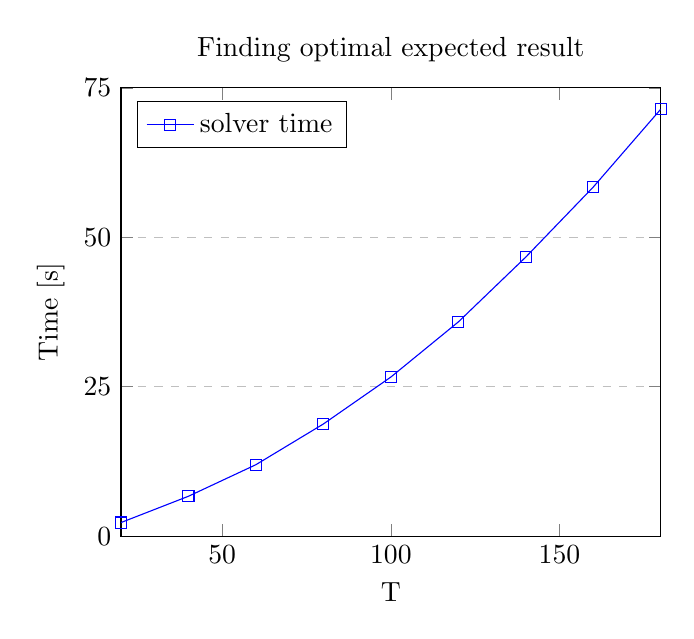
\begin{tikzpicture}
\begin{axis}[
    title={Finding optimal expected result},
    xlabel={T},
    ylabel={Time [s]},
    xmin=20, xmax=180,
    ymin=0, ymax=75,
    xtick={0,50,100,150,200},
    ytick={0,25,50,75},
    legend pos=north west,
    ymajorgrids=true,
    grid style=dashed,
]

\addplot[
    color=blue,
    mark=square,
    ]
    coordinates {
    (20,2.28)(40,6.68)(60,11.96)(80,18.77)(100,26.62)(120,35.84)(140,46.69)(160,58.40)(180,71.42)
    };
    \legend{solver time}

\end{axis}
\end{tikzpicture}
\end{subfigure}
\hfill
\begin{subfigure}[H]{0.4\textwidth}
	\centering
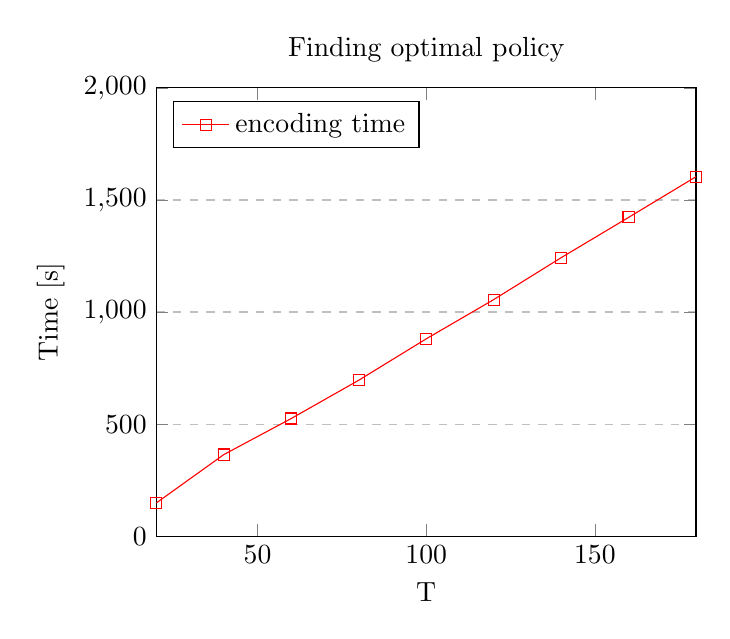
\begin{tikzpicture}
\begin{axis}[
    title={Finding optimal policy},
    xlabel={T},
    ylabel={Time [s]},
    xmin=20, xmax=180,
    ymin=0, ymax=2000,
    xtick={0,50,100,150},
    ytick={0,500,1000,1500,2000},
    legend pos=north west,
    ymajorgrids=true,
    grid style=dashed,
]
    
\addplot[
    color=red,
    mark=square,
    ]
    coordinates {
    (20,148.55)(40,364.16)(60,525.13)(80,695.75)(100,880.37)(120,1055.46)(140,1242.38)(160,1422.13)(180,1603.73)
    };
    \legend{encoding time}
    
\end{axis}
\end{tikzpicture}
\end{subfigure}
\caption{Results for $N=5$}
\end{figure}









\begin{figure}[H]
\centering
\begin{subfigure}[H]{0.4\textwidth}
	\centering

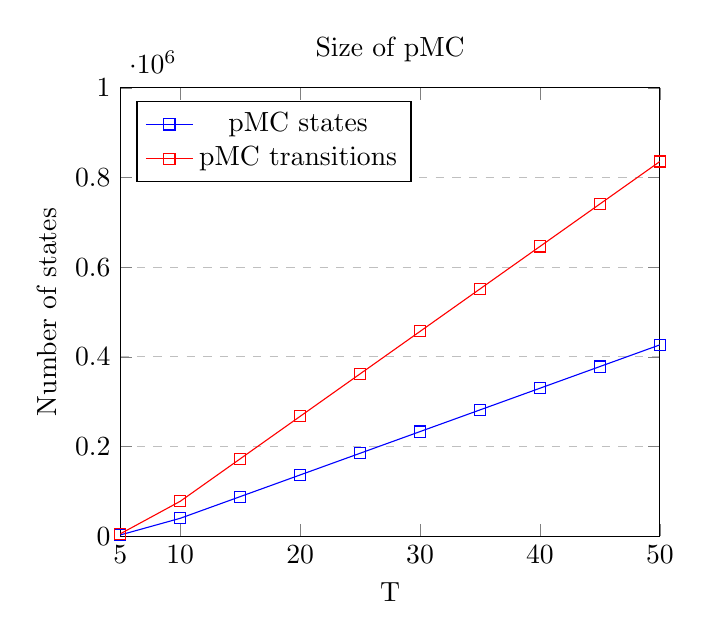
\begin{tikzpicture}
\begin{axis}[
    title={Size of pMC},
    xlabel={T},
    ylabel={Number of states},
    xmin=5, xmax=50,
    ymin=0, ymax=1000000,
    xtick={5,10,20,30,40,50},
    ytick={0,200000,400000,600000,800000,1000000},
    legend pos=north west,
    ymajorgrids=true,
    grid style=dashed,
]

\addplot[
    color=blue,
    mark=square,
    ]
    coordinates {
(5,2740)(10,39908)(15,88268)(20,136628)(25,184988)(30,233348)(35,281708)(40,330068)(45,378428)(50,426788)
    };
    
\addplot[
    color=red,
    mark=square,
    ]
    coordinates {
(5,5223)(10,77819)(15,172564)(20,267309)(25,362054)(30,456799)(35,551544)(40,646289)(45,741034)(50,835779)
    };
    \legend{pMC states, pMC transitions}
    
\end{axis}
\end{tikzpicture}
\end{subfigure}
\hfill
\begin{subfigure}[H]{0.4\textwidth}
	\centering
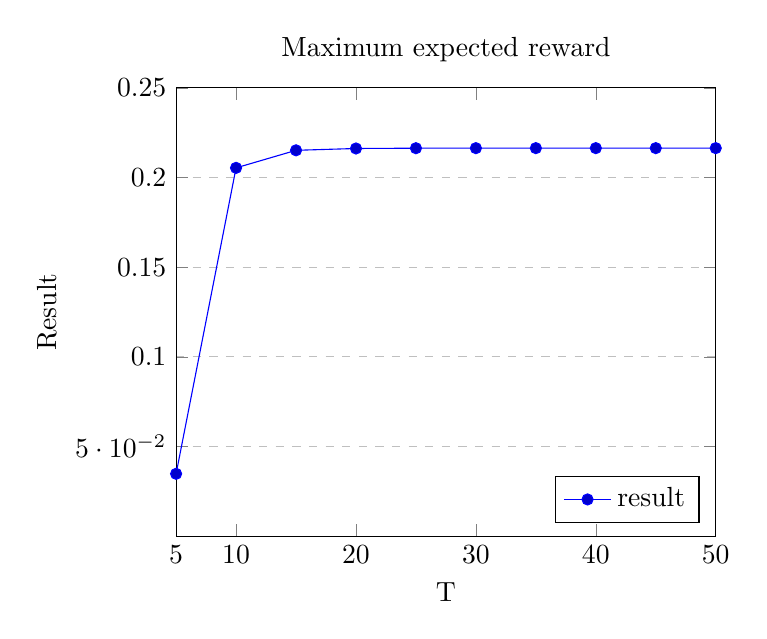
\begin{tikzpicture}

\begin{axis}[
    title={Maximum expected reward},
    xlabel={T},
    ylabel={Result},
    xmin=5, xmax=50,
    ymin=0, ymax=0.25,
    xtick={5,10,20,30,40,50},
    ytick={0.05,0.1,0.15,0.2,0.25},
    legend pos=south east,
    ymajorgrids=true,
    grid style=dashed,
]
    
\addplot
    coordinates {
(5,0.034790)(10,0.20539)(15,0.21518)(20,0.21620)(25,0.21636)(30,0.21639)(35,0.21640)(40,0.21640)(45,0.21640)(50,0.21640)
    };
    \legend{result}
    
\end{axis}
\end{tikzpicture}
\end{subfigure}

\begin{subfigure}[H]{0.4\textwidth}
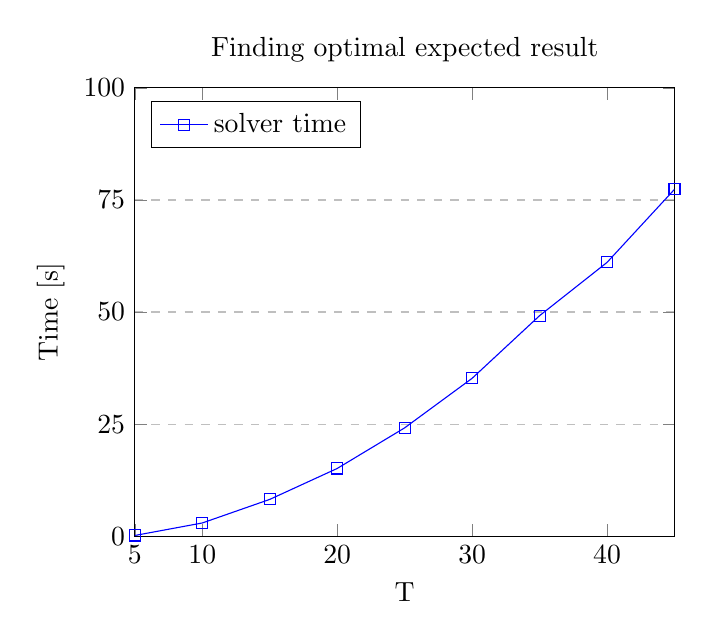
\begin{tikzpicture}
\begin{axis}[
	title={Finding optimal expected result},
    xlabel={T},
    ylabel={Time [s]},
    xmin=5, xmax=45,
    ymin=0, ymax=100,
    xtick={5,10,20,30,40,50},
    ytick={0,25,50,75,100},
    legend pos=north west,
    ymajorgrids=true,
    grid style=dashed,
]

\addplot[
    color=blue,
    mark=square,
    ]
    coordinates {
(5,0.16)(10,2.95)(15,8.21)(20,15.11)(25,24.17)(30,35.22)(35,49.19)(40,61.07)(45,77.37)
    };
    \legend{solver time}
    
\end{axis}
\end{tikzpicture}
\end{subfigure}
\hfill
\begin{subfigure}[H]{0.4\textwidth}
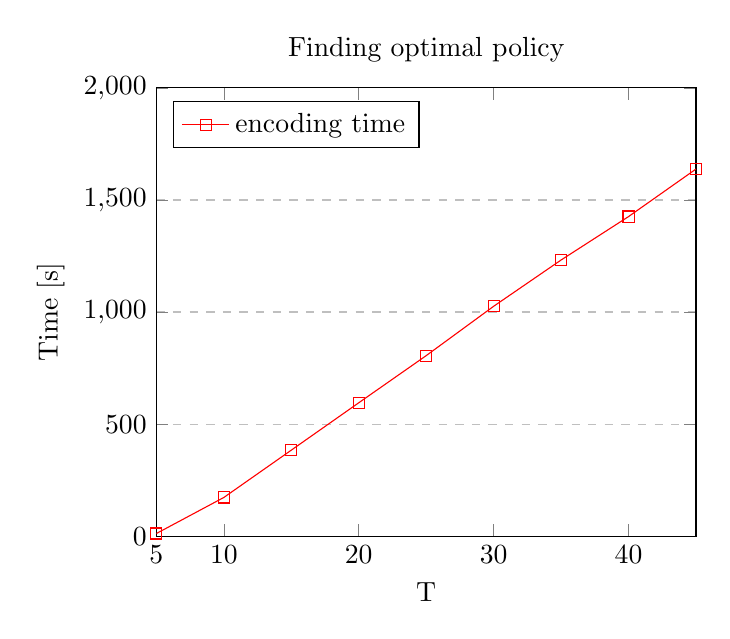
\begin{tikzpicture}
\begin{axis}[
title={Finding optimal policy},
    xlabel={T},
    ylabel={Time [s]},
    xmin=5, xmax=45,
    ymin=0, ymax=2000,
    xtick={5,10,20,30,40,50},
    ytick={0,500,1000,1500,2000},
    legend pos=north west,
    ymajorgrids=true,
    grid style=dashed,
]
    
\addplot[
    color=red,
    mark=square,
    ]
    coordinates {
(5,11.95)(10,172.79)(15,383.88)(20,595.19)(25,805.52)(30,1025.71)(35,1232.19)(40,1425.90)(45,1638.00)
    };
    \legend{encoding time}
    
\end{axis}
\end{tikzpicture}
\end{subfigure}
\caption{Results for $N=10$}
\end{figure}